ユーザによるファイルのアップロードを処理したいとします。例えば、現在Instagramのようなホームページを作成しているとします。ユーザが撮影した写真を保存する必要があります。このような要求はどのように実現するのでしょうか?

フォームにファイルをアップロードさせるためには、まずformの\texttt{enctype}属性を追加する必要があります。\texttt{enctype}属性には以下の3つの種類があります:


\begin{lstlisting}[numbers=none]
application/x-www-form-urlencoded
     送信前にすべての文字列をエンコードする(デフォルト)
multipart/form-data
     文字列に対してエンコードしません。
     ファイルのアップロードウィジェットを含む
     フォームを使用するときはこの値が必要です。
text/plain
     空白を"+"記号に置き換えます。
     ただし、特殊文字に対してエンコードは行われません。
\end{lstlisting}

そのため、フォームのhtmlコードはこのようになります:

\begin{lstlisting}[numbers=none]
<html>
<head>
    <title>ファイルアップロード</title>
</head>
<body>
<form enctype="multipart/form-data"
      action="http://127.0.0.1:9090/upload"
      method="post">
  <input type="file" name="uploadfile" />
  <input type="hidden" name="token" value="{{.}}"/>
  <input type="submit" value="upload" />
</form>
</body>
</html>
\end{lstlisting}

サーバでは、handlerFuncをひとつ追加します:

\begin{lstlisting}[numbers=none]
http.HandleFunc("/upload", upload)

// /uploadを処理するロジック
func upload(w http.ResponseWriter, r *http.Request) {
    fmt.Println("method:", r.Method) //リクエストを受け取るメソッド
    if r.Method == "GET" {
        crutime := time.Now().Unix()
        h := md5.New()
        io.WriteString(h, strconv.FormatInt(crutime, 10))
        token := fmt.Sprintf("%x", h.Sum(nil))

        t, _ := template.ParseFiles("upload.gtpl")
        t.Execute(w, token)
    } else {
        r.ParseMultipartForm(32 << 20)
        file, handler, err := r.FormFile("uploadfile")
        if err != nil {
            fmt.Println(err)
            return
        }
        defer file.Close()
        fmt.Fprintf(w, "%v", handler.Header)
        f, err := os.OpenFile("./test/"+handler.Filename,
                              os.O_WRONLY|os.O_CREATE, 0666)
        if err != nil {
            fmt.Println(err)
            return
        }
        defer f.Close()
        io.Copy(f, file)
    }
}
\end{lstlisting}

上のコードでは、ファイルのアップロードを処理するためには\texttt{r.ParseMultipartForm}をコールする必要があります。引数には\texttt{maxMemory}が表示されています。\texttt{ParseMultipartForm}をコールした後、アップロードするファイルは\texttt{maxMemory}のサイズのメモリに保存されます。もしファイルのサイズが\texttt{maxMemory}を超えた場合、残った部分はシステムのテンポラリファイルに保存されます。\texttt{r.FormFile}によって上のファイルハンドルを取得することができます。その後実例の中では\texttt{io.Copy}を使ってファイルを保存しています。

\begin{quote}
その他のファイルではないフィールド情報を取得する時は\texttt{r.ParseForm}をコールする必要はありません。必要な時はGoが自動でコールします。また\texttt{ParseMultipartForm}を一度コールすると、その後にもう一度コールしても効果はありません。
\end{quote}

上の実例を通して、ファイルのアップロードには主に3ステップの処理があることが分かります:

\begin{enumerate}
  \item フォームにenctype="multipart/form-data"を追加する。
  \item サーバで\texttt{r.ParseMultipartForm}をコールし、アップロードするファイルをメモリとテンポラリファイルに保存する。
  \item \texttt{r.FormFile}を使用して、ファイルハンドルを取得し、ファイルに対して保存等の処理を行う。
\end{enumerate}

ファイルhandlerはmultipart.FileHeaderです。この中には以下のような構造体が保存されています。

\begin{lstlisting}[numbers=none]
type FileHeader struct {
    Filename string
    Header   textproto.MIMEHeader
    // contains filtered or unexported fields
}
\end{lstlisting}

上のコード例では以下のようにファイルのアップロードを出力します。

\begin{figure}[H]
  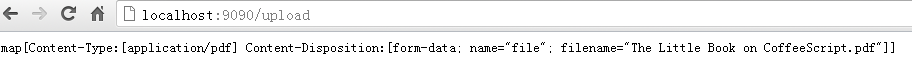
\includegraphics[width=14cm]{4.5.upload2.png}
   \label{図4.5}
   \caption{ファイルのアップロードを行った後サーバが受け取った情報の出力}
\end{figure}
